
% Inbuilt themes in beamer
\documentclass{beamer}

% Theme choice:
\usetheme{Warsaw}

%package
\usepackage{hyperref}

% Title page details: 
\title{On the misuse of regressions of price on
the HHI in merger review} 
\subtitle{Nathan Miller et al\\ \textit{Journal of Antitrust Enforcement 2022}}
\author{Presented by: Ka Yan CHENG}
\date{ \vspace*{-1cm}\\ ECON 771 Health Economics II, Fall 2022}

% Fix the footline too long problem
\setbeamertemplate{headline}{}
\setbeamertemplate{footline}{%
  \leavevmode%
  \hbox{\begin{beamercolorbox}[wd=.5\paperwidth,ht=4.5ex,dp=2.125ex,leftskip=.3cm plus1fill,rightskip=.3cm]{author in head/foot}%
    \usebeamerfont{author in head/foot}\insertshortauthor
  \end{beamercolorbox}%
  \begin{beamercolorbox}[wd=.5\paperwidth,ht=4.5ex,dp=2.125ex,leftskip=.3cm,rightskip=.3cm plus1fil]{title in head/foot}%
    \usebeamerfont{title in head/foot}
    \parbox{.45\paperwidth}{\inserttitle}
  \end{beamercolorbox}}%
  \vskip0pt%
}

% Change subtitle format
\setbeamercolor{subtitle}{fg=lightgray}%
\setbeamerfont{subtitle}{size=\scriptsize}%



\setbeamerfont{date}{size=\footnotesize}


\begin{document}

% Title page frame
\begin{frame}
    \titlepage 
\end{frame}

% Remove logo from the next slides
\logo{}


% Outline frame
\begin{frame}{Outline}
    \tableofcontents
\end{frame}


% Lists frame
\section{Motivation}

\begin{frame}{Motivation}
\framesubtitle{Role of HHI on merger review}
The Herfindahl-Hirschman Index (HHI) measures market concentration by taking the form of:\\
\begin{equation*}
HHI = 10000 \times \sum_n s_n^2
\end{equation*}
where $s_i = \frac{q_i}{Q}$ indicates the market share of each firm $i$.\\
\hfill \break
For example, for  a market with 3 firms that own output shares of $40\%$, $30\%$ and $30\%$:
\begin{equation*}
HHI = 40^2 + 30^2 + 30^2 = 3400 
\end{equation*}
HHI = 0: Perfect competition\\
HHI = 10000: Monopoly market
\end{frame}

\begin{frame}{Motivation}
\framesubtitle{Role of HHI on merger review}
Connecting HHI with merger
\begin{itemize}
\item All else equal, decrease in number of firms leads to a higher HHI
\item Given same amount of firms, HHI increases when the market share of larger firms increase
\item The implied change in HHI after merger of firm $i$ and $k$:
$$\Delta HHI  = 2 \times s_i \times s_k$$
\end{itemize}
\end{frame}

\begin{frame}{Motivation}
\framesubtitle{Role of HHI on merger review}
Merger review
\begin{itemize}
\item Goal: identify and prevent  mergers that are more likely to have anticompetitive effects (raise price, reduce output)
\begin{center}
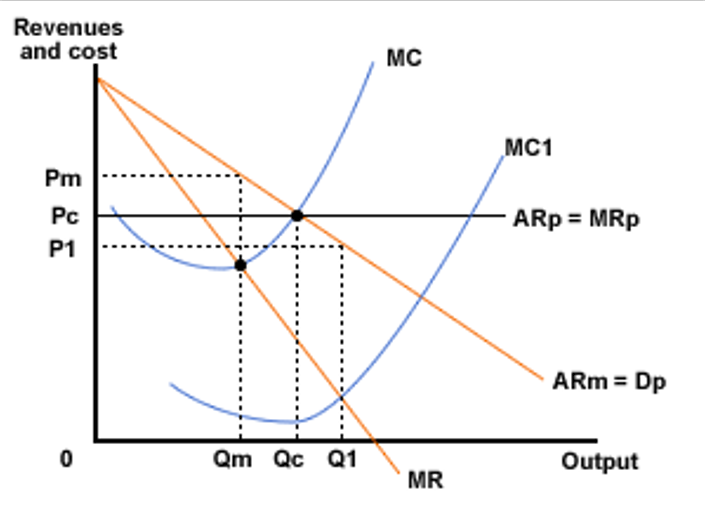
\includegraphics[height=4.5cm]{pic188}
\end{center}
 \begin{flushright}
\href{http://www.sanandres.esc.edu.ar/secondary/economics\%20packs/microeconomics/page_121.htm}{[Souce of figure]}
\end{flushright} 
\item Question of interest: \\
Causal impact of \textbf{mergers} on price
\end{itemize}
\end{frame}

\begin{frame}{Motivation}
\framesubtitle{Relationship between price and HHI}
HHI on merger review in practice
\begin{enumerate}
\item The Horizontal Merger Guidelines of the US Department of Justice and Federal Trade Commission (2010)\\
	\begin{itemize}
	\item Mergers that generate a \textbf{post-merger HHI above 2500} and \textbf{increase in the HHI by 200 or more} "will be presumed to be likely to enhance market power"
	\end{itemize}
\item Courts in the state
\item Merger guidelines of the European Union
\end{enumerate}
\hfill \break
\end{frame}

%Reseach question
\section{Main question}
\begin{frame}{Main question}
\begin{center}
Causal impact of \textbf{mergers} on price\\ 
v.s.\\
 Causal impact of \textbf{HHI} on price
\end{center}
\end{frame}

%Contribution
\section{Contribution}
\begin{frame}{Contribution}
To explain why regressions of price on the HHI should \textbf{NOT} be used in merger review
\end{frame}

%Preview of findings
\section{Preview of findings}
\begin{frame}{Preview of findings}
\begin{center}
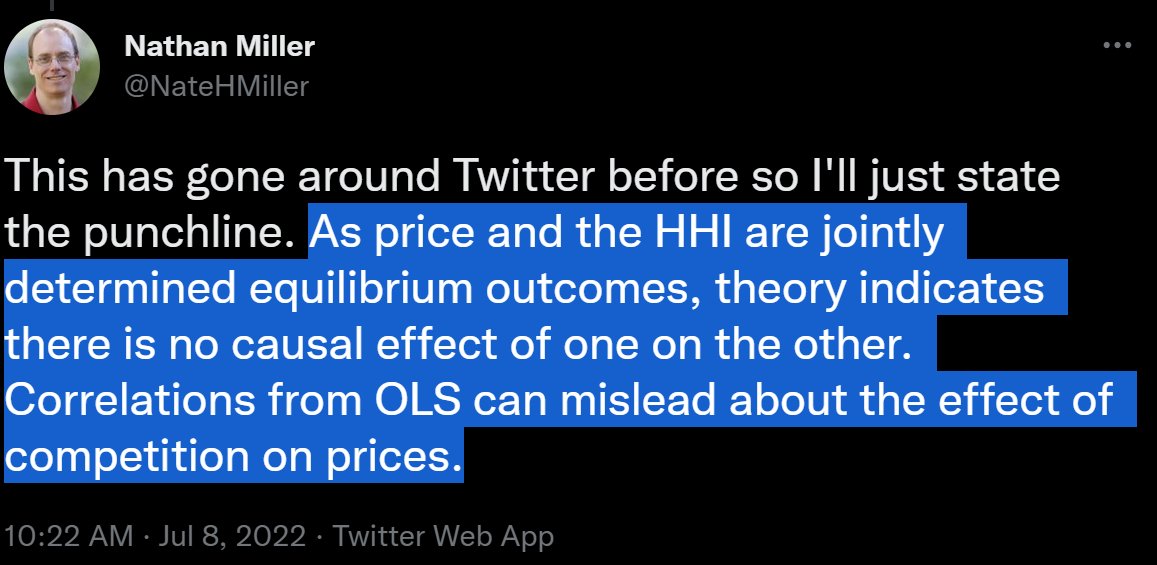
\includegraphics[height=4.5cm]{nathanmillertwit}
\end{center}
\end{frame}

%Data
\section{Methodology}
\begin{frame}{Methodology}
Provide simple numerical examples to demonstrate
\begin{enumerate}
\item Empirical price-HHI relationship is not useful for telling the competitive effects of mergers in general
\item The exceptional case that the former statement would not be true
\end{enumerate}
More like a guidebook, no data has been used.
\end{frame}

%Results
\section{Results}
\begin{frame}
\begin{center}
Results
\end{center}
\end{frame}

\begin{frame}{Numerical example of misleading price-HHI comparison}
\framesubtitle{Why it might not work well?}
Setup of the numerical example: (Cournot competition model) \\
Let the market inverse demand be $P(Q) = 10 - Q$,  and let there be $n = 1,2, \dots, N$ firms. In the equilibrium, the output of firm $i$ is given by
$$
q_i =  \frac{10-c_i+N(\bar{c} - c_i)}{(N+1)}
$$
where $c_i$ is the marginal cost of firm $i$ and $\bar{c} = \frac{1}{N}\sum_{N}c_n$ is the average marginal cost. The equilibrium price is 
$$
P = \frac{10+N\bar{c}}{N+1}
$$ 
And the equilibrium market quantity is 
$$
Q = \sum_n q_n = \frac{N(10-\bar{c})}{(N+1)}
$$
\end{frame}

\begin{frame}{Numerical example of misleading price-HHI comparison}
\framesubtitle{Why it might not work well?}
Consider $N=2$ firms that produce a homogenous good in 3 different regions which they have different margianl costs in production:
\begin{center}
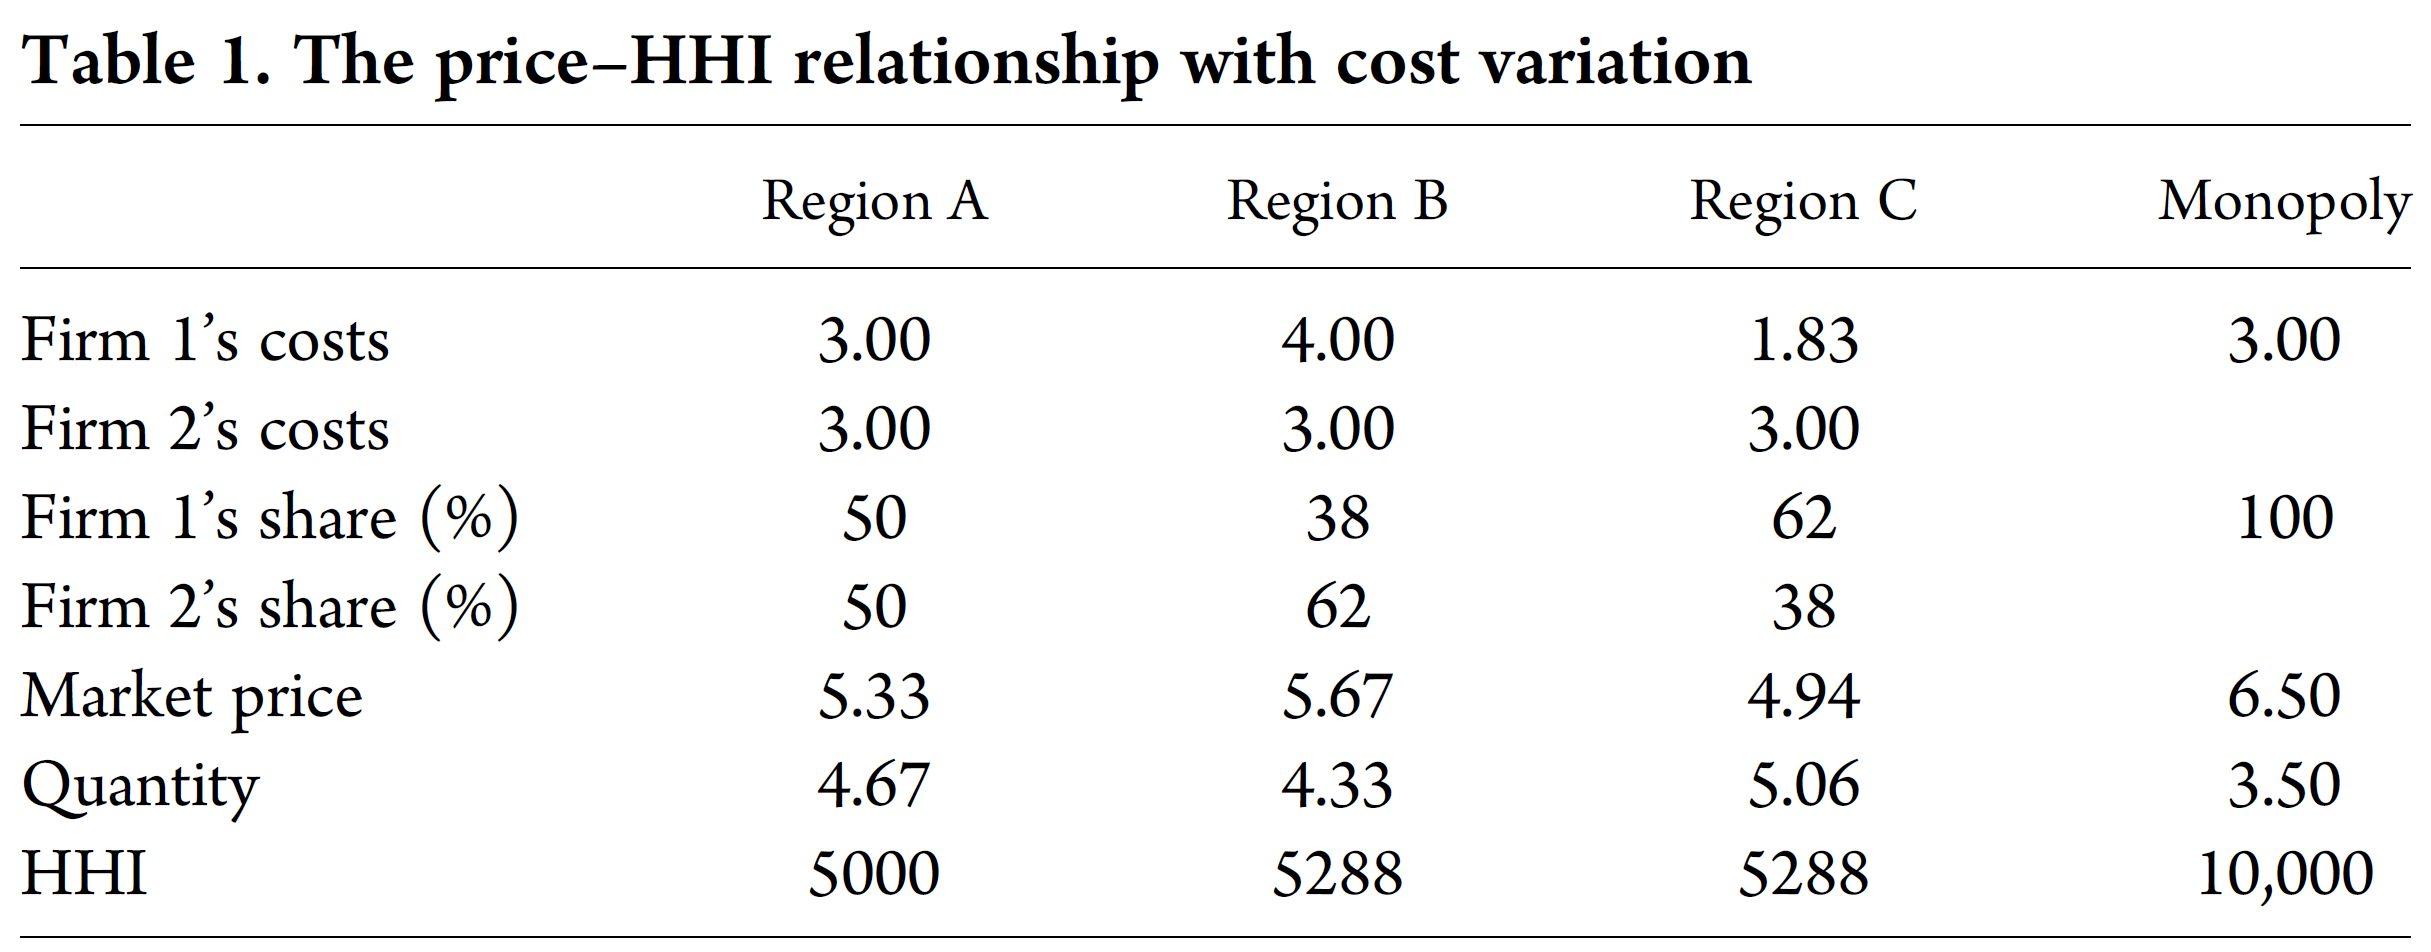
\includegraphics[height=4cm]{Tab1}
\end{center}
Comparing columns 1,2,3 with column  4 one by one, we can see the correlation between price and the HHI is ambiguous.
\end{frame}

\begin{frame}{Regressions of price on the HHI}
\framesubtitle{What is the problem?}
Typical form of a price on HHI regression model:\\
\begin{equation*}
P_i = \beta_0 + \beta_1\text{HHI}_{i} + \beta_2x_i + \epsilon_i
\end{equation*}
Again, our numerical example:
\begin{center}
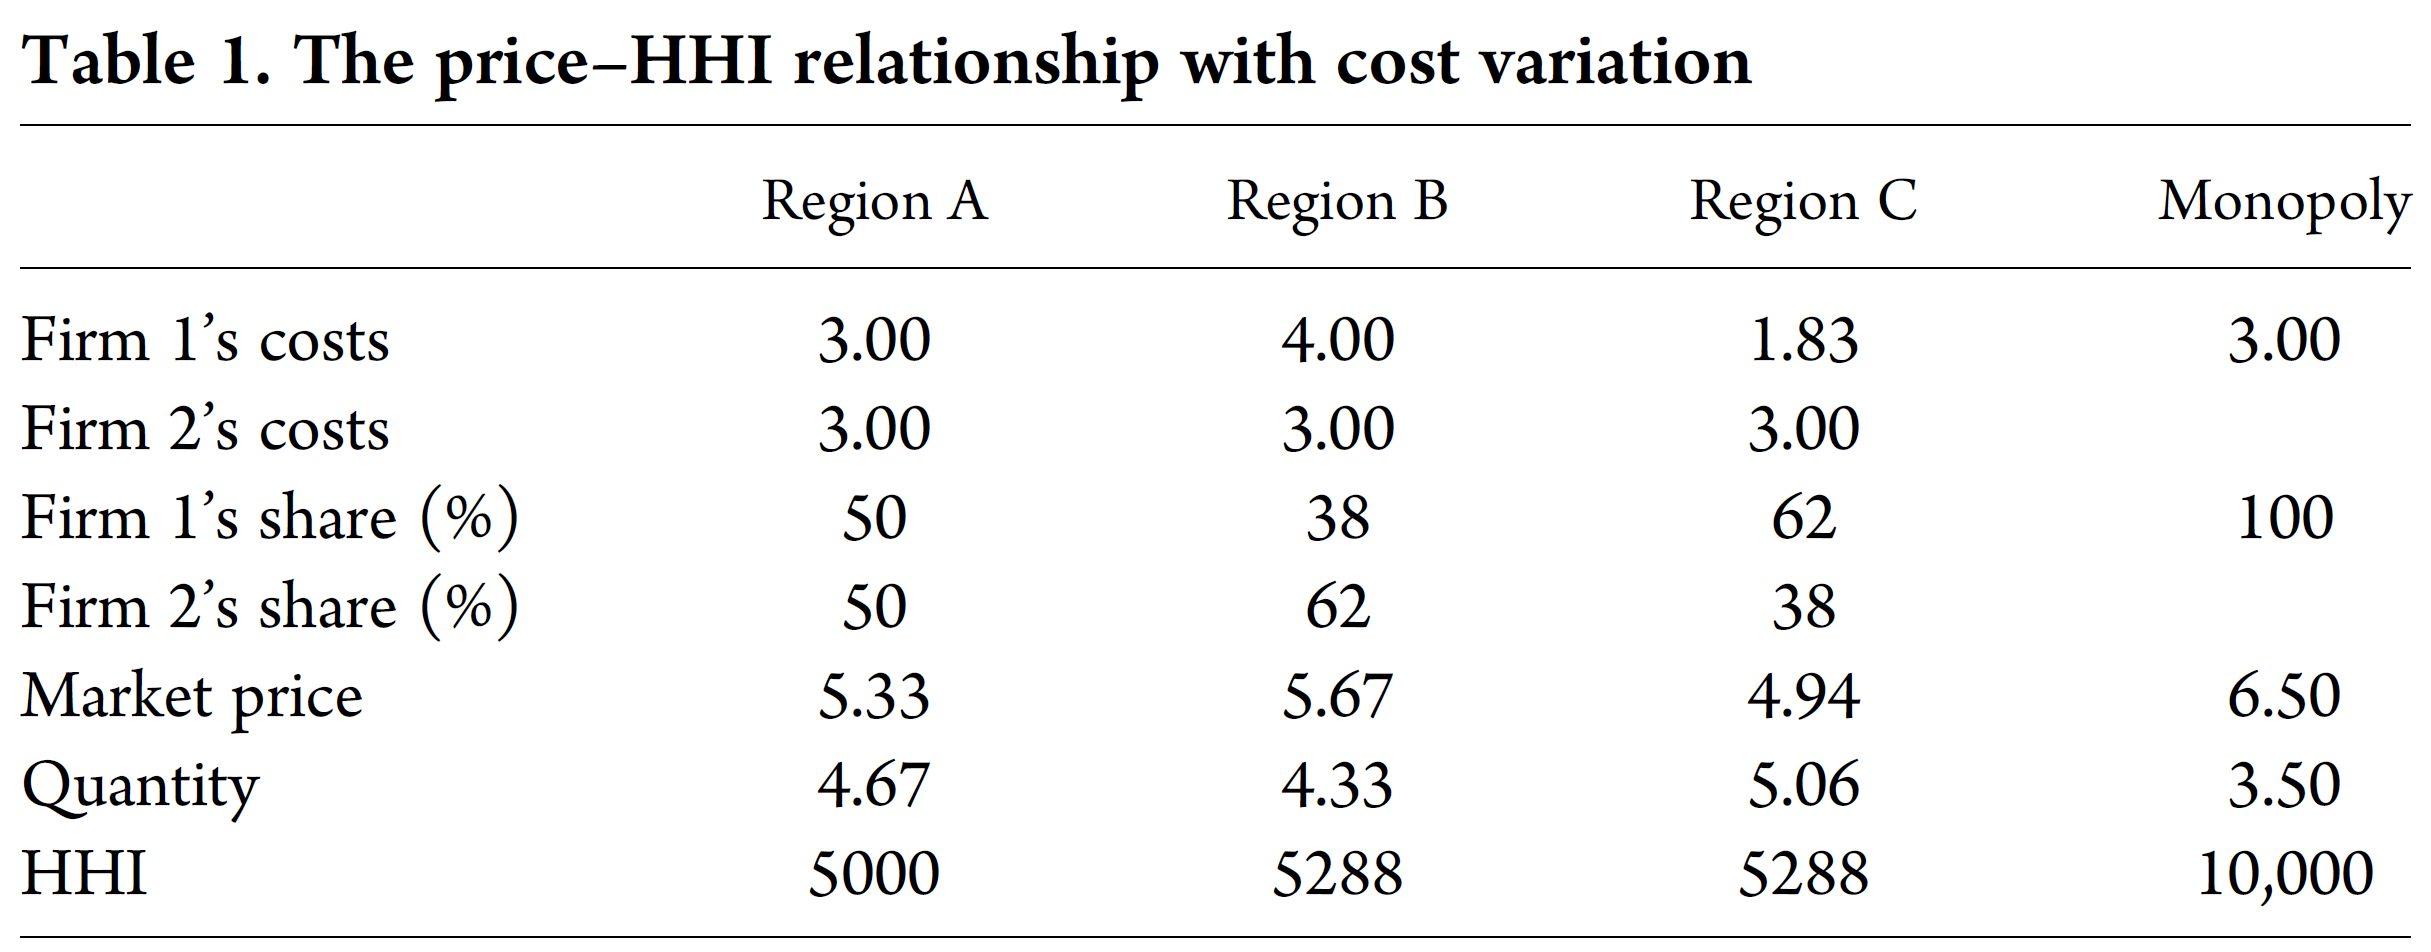
\includegraphics[height=4cm]{Tab1}
\end{center}
If we run a regression of price on the HHI based on the data of all 3 regions, we will get a slightly negative relationship.
\end{frame}

\begin{frame}{Regressions of price on the HHI}
\framesubtitle{What is the problem?}
The problem:
\begin{enumerate}
\item Both price and the HHI are market equilibrium outcomes. They are jointly determined in the equilibrium and there is no causal effect of one on the other.
\item Different estimate of the regression coefficient can pick up various possible correlations that exist due to variation in the underlying demand and supply factors, but \textbf{CANNOT} measure a causal effect that \textbf{DOES NOT} exist.
\end{enumerate}
\end{frame}

\begin{frame}{Appropriate role of the HHI in merger review}
\framesubtitle{How should we use it?}
A special case: \\
Empirical variation in the HHI is driven pedominantly by changes in competition
\end{frame}

\begin{frame}{Appropriate role of the HHI in merger review}
\framesubtitle{How should we use it?}
Now consider constant marginal cost $c = 3$ for all firms, and consider markets with different number if competitiors:
\begin{center}
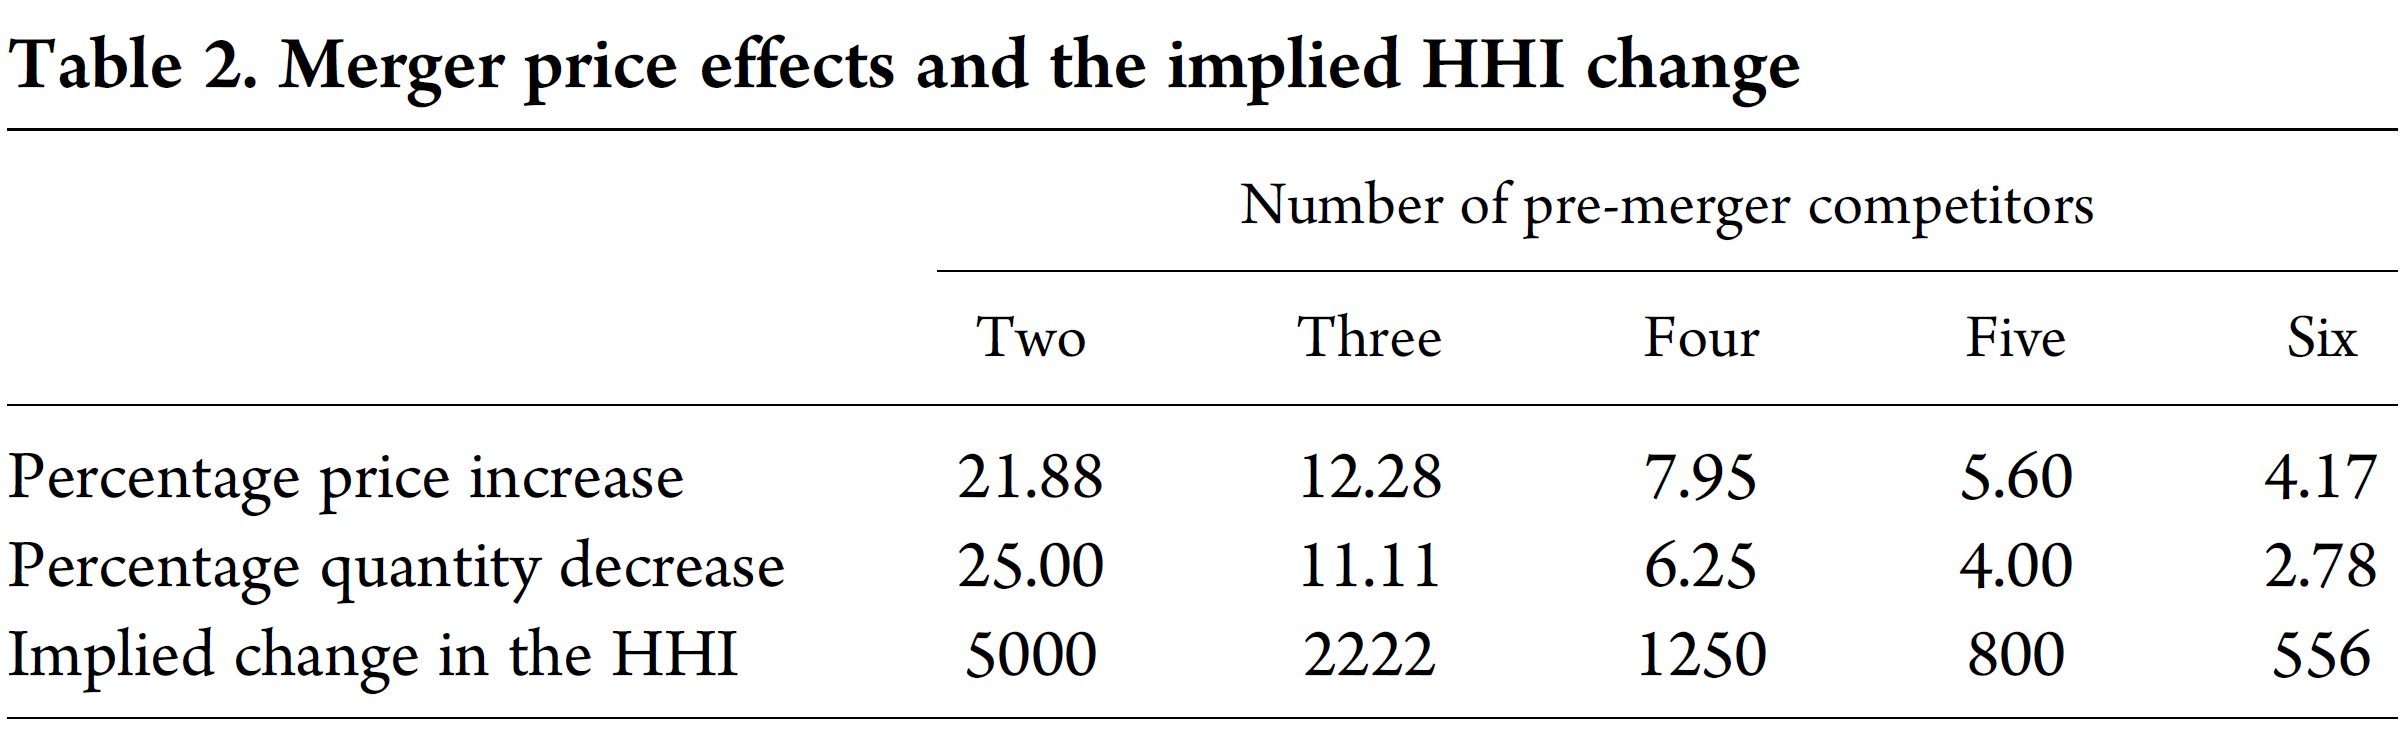
\includegraphics[height=3cm]{Tab2}
\end{center}
Relationship between the HHI and the price is still not causal, but the correlation in such special case can at least provide information on the impact of a merger on price.\\
\hfill \break
But in such case, just analyse directly the impact on prices from the merger event instead of the one that has been mediated through the HHI.
\end{frame}

%Threats
\section{Discussions}
\begin{frame}{Discussions}
What would be other better ways to empirically quantify the  causal impact of \textbf{mergers} on price/output level?
\end{frame}

%Results
\section{Conclusion}
\begin{frame}{Conclusion}
Regression of price on the HHI does not provide useful information on antitrust review of mergers as there is $\textbf{NO}$ causal relationship between the two.
\end{frame}

\end{document}